\documentclass{article}
\usepackage[utf8]{inputenc}
\usepackage{amsmath}
\usepackage{amsfonts}
\usepackage{amssymb}
\usepackage{graphicx}

\title{Models of Non-linear Dynamics and a Practical Demonstration.}
\author{{Yuan Yuxuan  u6772166 lab partner:Lu Tianshi u5861479}}
\date{}
\begin{document}

\maketitle
\textbf{ABSTRACT}

In our standard courses, we usually learn the pendulum whose motion is linear. But nonlinear motion of pendulum is also of great importance. Compared to solve the equations analytically in linear cases, we usually use the numerical method to solve and analysis the nonlinear equations and analysis the various properties of it.

\section{\textbf{INTRODUCTION}}

In this lab, we mainly deal with the inverted pendulum, the motion of which satisfy the duffing equation(a nonlinear equation). We do both the experiment and simulation and then compare them. In the remainder of this report, I derive the duffing equation for inverted pendulum(Section 2) and describe our experiment and results(Section 3). Then I present our numerical simulation of the system and carefully analysis them(Section 4). In the final I give our conclusion(Section 5). The relevant Mathematica code is also provided in appendix.


\section{\textbf{DUFFING EQUATIONS FOR INVERTED PENDULUM}}

The general form of the duffing equation is:
\begin{equation}
\ddot{x}+\delta\dot{x}+\alpha x+\delta x^3 = \gamma\cos(\omega t)
\end{equation}[2]
Now I will derive the duffing the equation for the inverted pendulum. There are gravity, restoring force, damping force and driving force exerted on inverted pendulum. From Newton's second Law we have:
\begin{equation}
ma = mg\sin(\phi) + A\sin(\omega t)-k\phi-k'\dot{\phi}
\end{equation}
Using $a = l\ddot\phi$ and Taylor expansion $\sin(\phi) = \phi - \phi^3/6$(where I neglect all the higher order term), we get:
\begin{equation}
ml\ddot{\phi} + \gamma\dot{\phi} + (k-mg)\phi +\frac{mg}{6}\phi^3=  A\sin(\omega t)
\end{equation}
Which is duffing equation, explicitly.


\section{\textbf{EXPERIMENTS}}

Experimental equipments is shown in fig 1, including Optical table, clamps, Stanford function generator, magnet,ultrasonic sensor, PC. We adjust our equipment to find proper driven force and position for the mass. The systems' motion is nonlinear but its motion is within the boundary that we set. We record the motion by using the ultrasonic sensor linked to PC[1].
\begin{figure}[h]
	\centering
	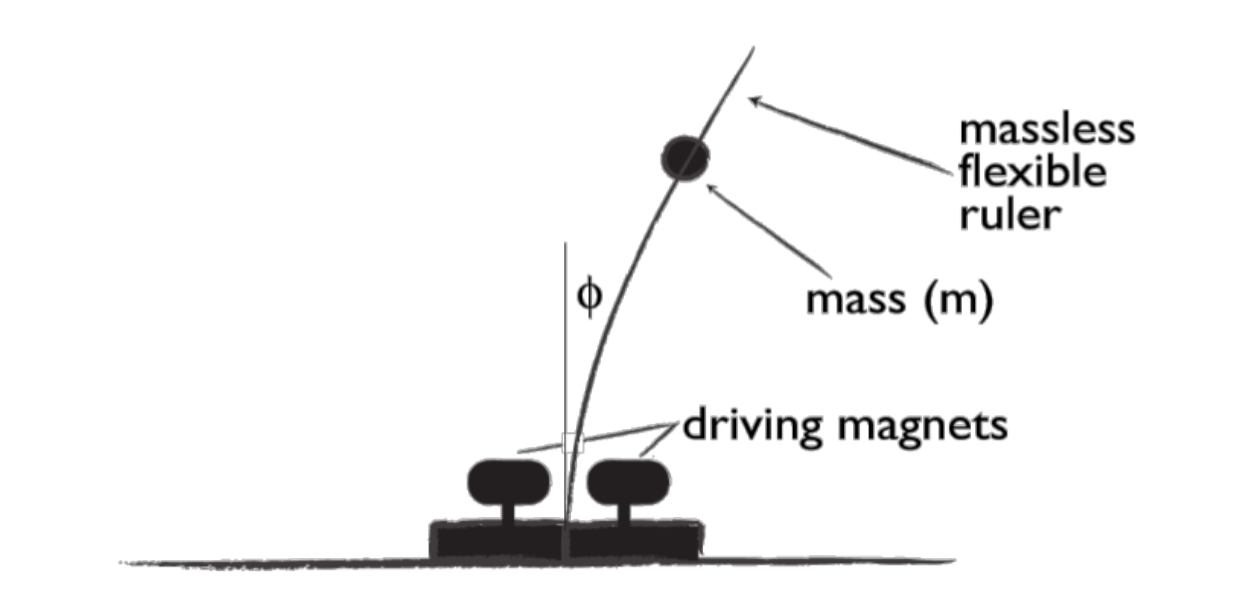
\includegraphics[width=0.7\linewidth]{plot/exp}
	\caption{experimental equipment}
	\label{fig:exp}
\end{figure}

Our experimental results is shown in fig 2. We choose three sets of plots. each set contains a phase plot and a time series plot of position versus time. In phase plot, x axis stands for position(m), while y axis stands for velocity(cm/s). The units in time series plot are s and m, respectively.
The difference of each set is the driving force, which is modified by voltage of the equipment. When U=3V or 4.5V, the system is in linear regime and will converge to small sinusoidal oscillation around one of the equilibrium position, which is around 0.19m or 0.31m. When U=8.7V, the system is in chaotic regime, and the system will move back and force around two equilibrium positions. 
\begin{figure}[h]
	\centering
	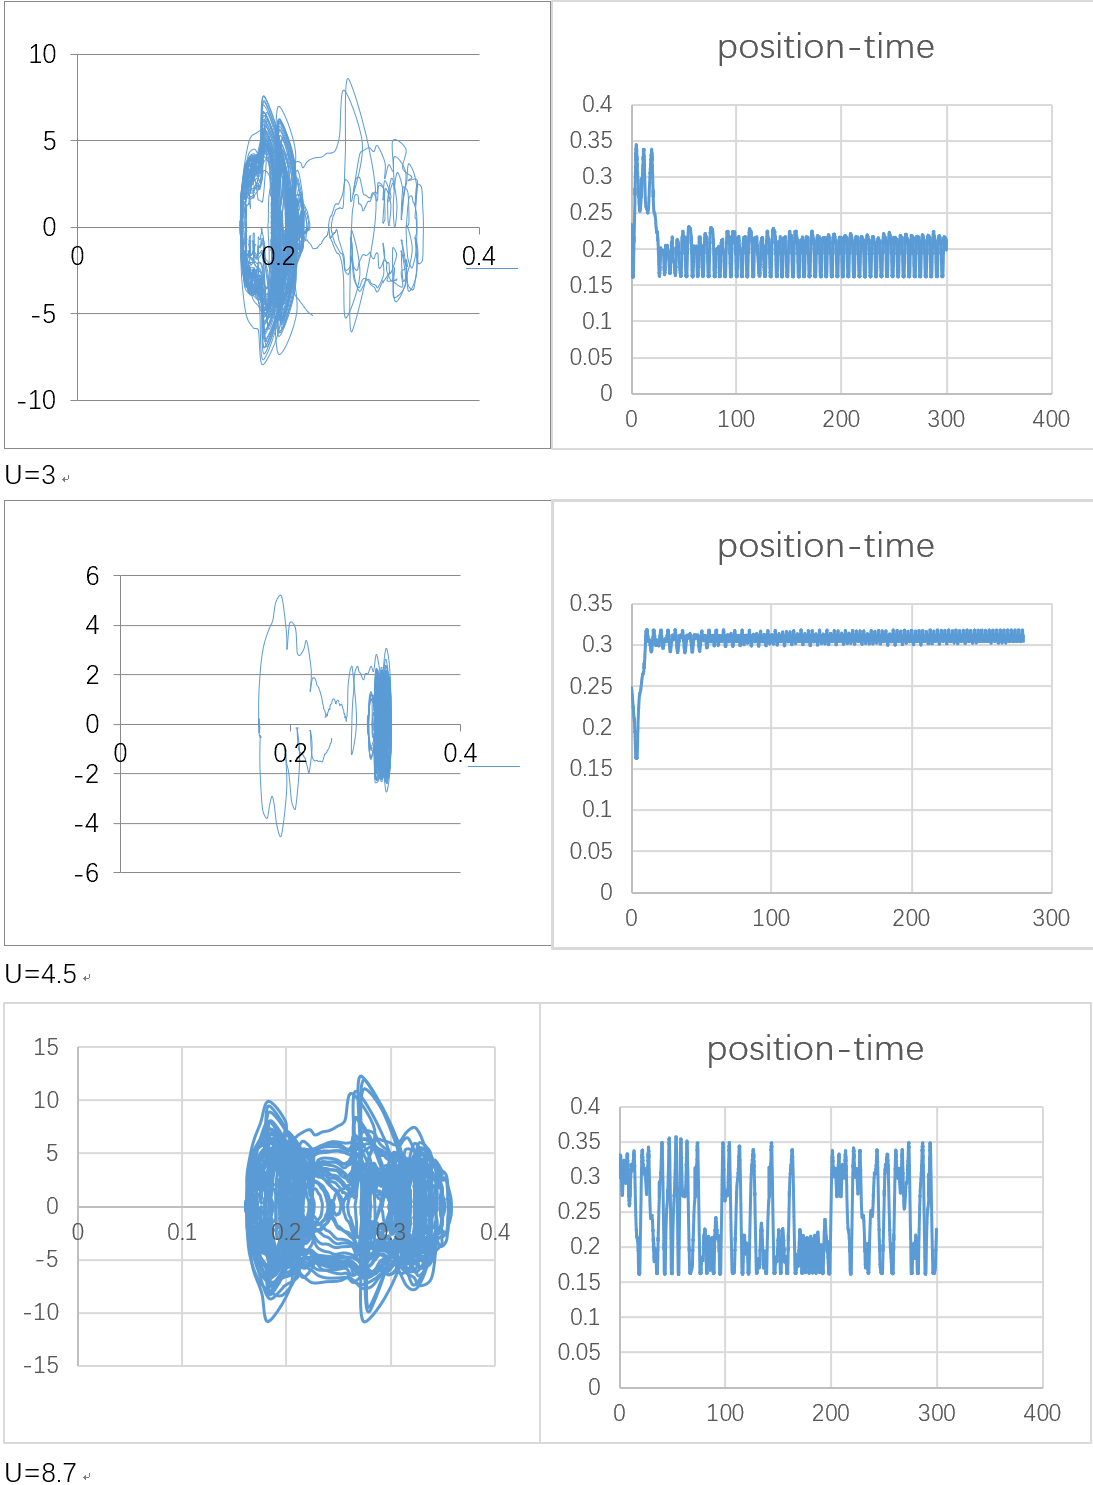
\includegraphics[width=0.7\linewidth]{plot/exp_res}
	\caption{experimental results}
	\label{fig:expres}
\end{figure}




\section{\textbf{NUMERICAL SIMULATIONS}}

In this lab, we use Mathematica to do the simulation. Our simulation include four parts, the first is Data visualization, which contain Phase Plot, Time-series plot; the second is Poincaré section; the third is basins of attraction; and the fourth is plot of Periodic doubling. The units in these plots for different quantities are: position(angle):rad; velocity:rad/s; time:s; Amplitude(A):N. I will omit the unit below for simplicity.


\subsection{\textbf{Data visualizations}}

In this part, I will give three sets of parameters. The difference for these three sets will only be the amplitude of the driven force(A), for that it affects the nonlinear behavior of the motion. All three sets set $m=0.235$, $l=0.22$, $\gamma=0.01$, $k=0.05$, $g=9.8$ and the amplitude(A) for three sets will be 0.1,1,3, respectively. The phase plots and time-series plots for each set are shown in fig 3, and the blue lines represent position while yellow lines represent velocity in time-series plot. We can see clearly that the behaviors of each set are different. When A is 0.1 or 1, the system is linear, so it will go into simple damping oscillation as time goes on. When A is 3, the system is chaotic so its behavior will become unpredictable and irregular. We can see that there are two equilibrium positions on each side, as the system will converge to one of them when A is small and will go around these two positions when A is large.

\begin{figure}[H]
	\centering
	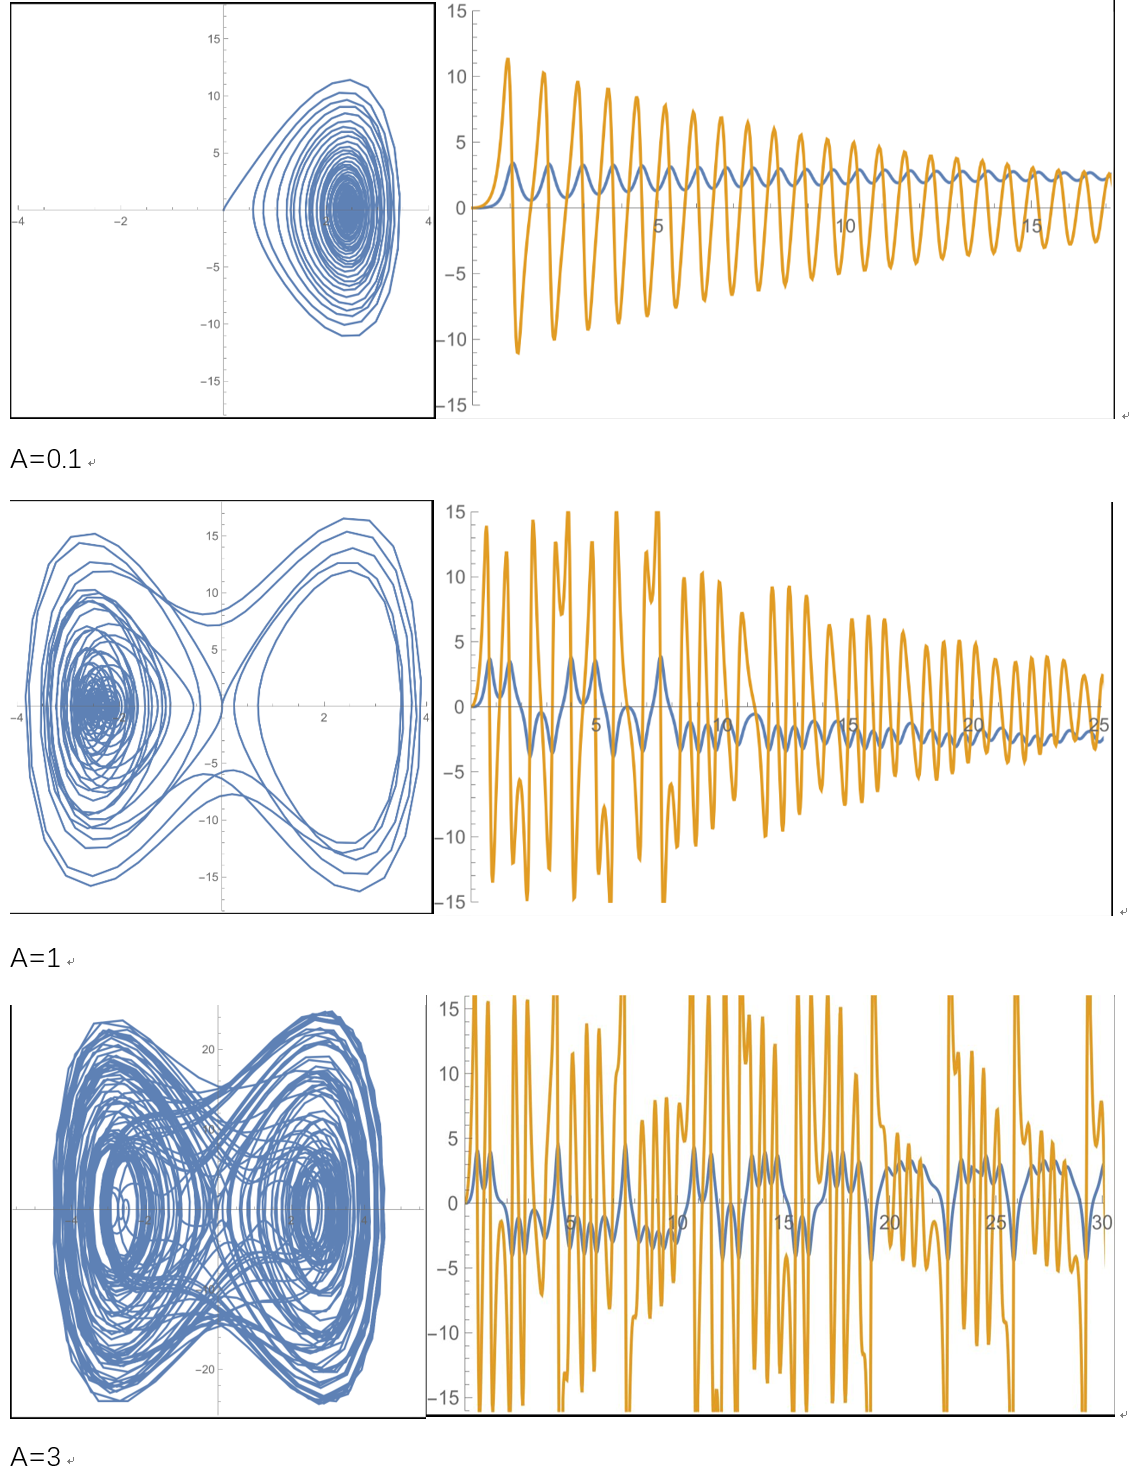
\includegraphics[width=0.7\linewidth]{plot/vis}
	\caption{visualization}
	\label{fig:vis}
\end{figure}

\subsection{\textbf{Poincaré Section}}
Then I will show you the Poincaré section. The x and y axis of Poincaré section plot are the same with the phase plot, but the difference between them is that the Poincaré section draw a point per period of driving force, while phase plot draw a curve for continuous time series. The Poincaré sections are shown in fig 4.[2]
\begin{figure}[h]
	\centering
	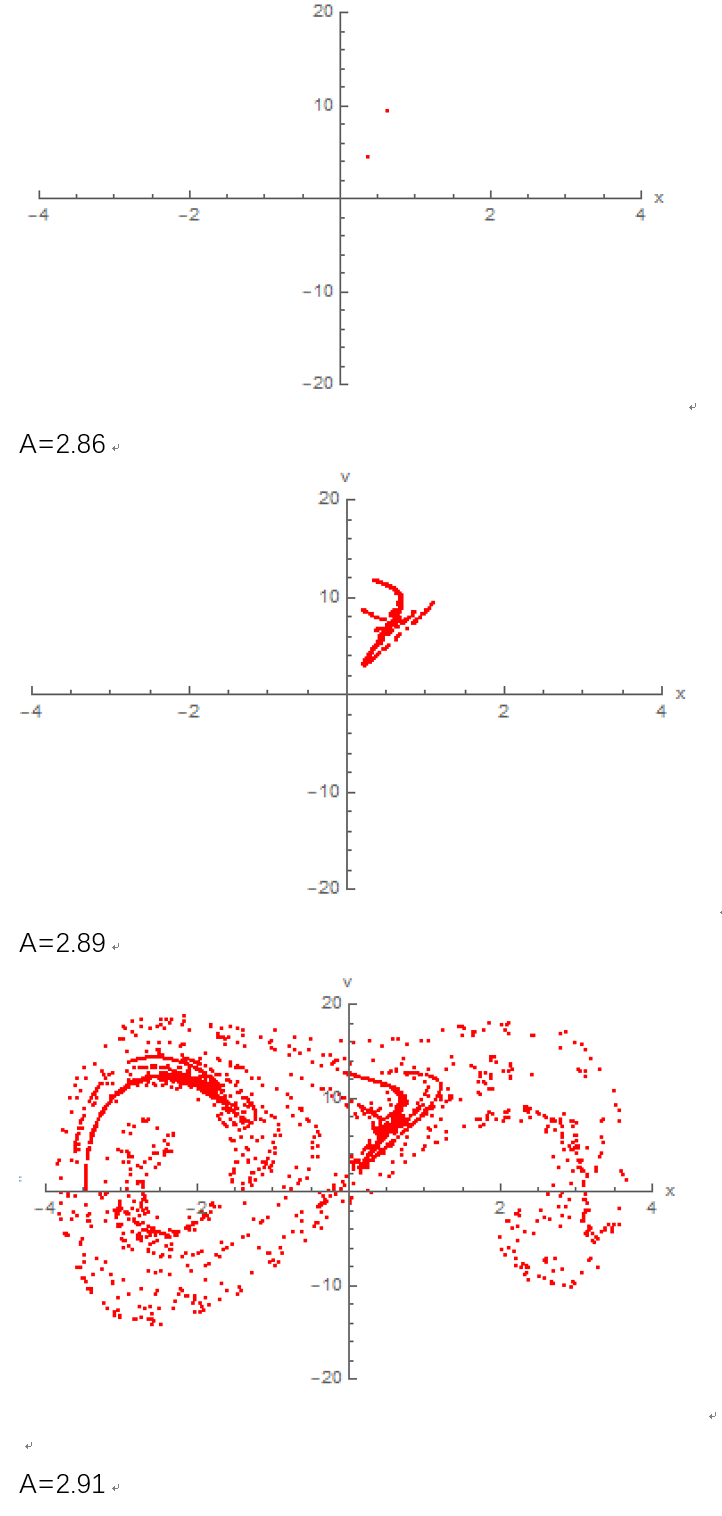
\includegraphics[width=0.5\linewidth]{plot/poincare}
	\caption{Poincaré section}
	\label{fig:poincare}
\end{figure}

This time the set of amplitudes will differ from the ones above, in order to show that there is a transition regime between linear and chaotic regime and a critical point which separate the transition regime and chaotic regime. When A is 2.86, due to the linear behavior of the system, it will give different phase point per period at the beginning of the time but then will give almost the same phase point per period, as shown in the first plot in fig 4. Then, when A is 2.89, the system is between linear and chaotic,namely in transition regime, and it will give different phase point per period, but still in a certain small region in phase space, as shown in the second plot. Lastly, when A is 2.91, the system is chaotic, and the phase points will spread over a much bigger region in phase space, as shown in the last plot. The changes in these three plot show that the critical point is between 2.89 and 2.91. And in section 5.3 periodic doubling, we will study the critical phenomena of the system more deeply and precisely get the critical point.


\subsection{\textbf{Basin of attraction}}
If A is close to the transition regime, The system will eventually oscillate around one of the equilibrium point after a long enough time. And this results are highly sensitive to the initial condition. We found that amplitudes of 2.75,2.9 and 3 are appropriate for making basin of attraction as it is close to the transition regime. We plot it over the initial value phase space(where x axis stands for initial position and y axis stands for initial velocity), and red points means that the system eventually will go around the positive stable point, while blue point means the opposite.[4] Three basin of attraction are shown in fig 5.

\begin{figure}[h]
	\centering
	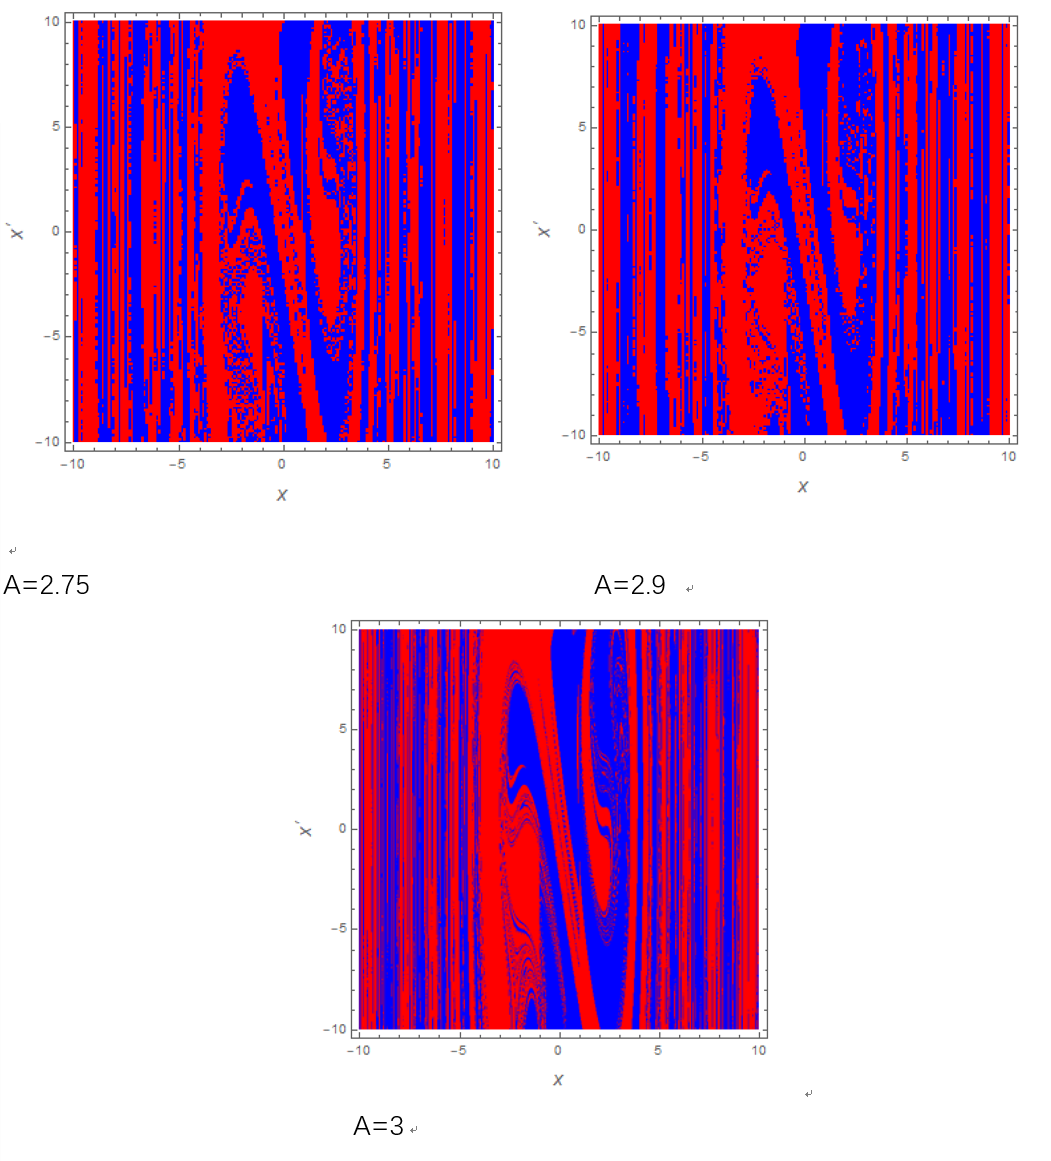
\includegraphics[width=0.5\linewidth]{plot/basin_2}
	\caption{basin of attraction}
	\label{fig:basin}
\end{figure}

We can see two things from this plot. First, the system is highly sensitive to the initial condition. Any tiny change in initial condition will lead to changes in motion afterward, hence oscillate around different equilibrium points. Second, the basin of attraction of these A are quite similar, as A is close to the transition region.

\subsection{\textbf{Periodic doubling}}
In order to show the transition between linear and chaotic behavior more clearly, we use bifurcation plot. The period of motion is dependent on the value of A. The period corresponding to small A is the same with the period of the driving force($2\pi/\omega$). But as A increases, the period of motion will double($4\pi/\omega,8\pi/\omega$,...) at some certain points and will goto chaotic regime at the critical point. As a sequence, If we plot the position per period($2\pi/\omega$) versus A after long enough time, we will get one point when the period of motion is $2\pi/\omega$, two points when it is $4\pi/\omega$, four when $8\pi/\omega$,etc. And it will goto chaotic regime in the last.[1]

The bifurcation plot is shown in fig 6.[2] We can see that the transition regime is nearly between 2.88$\pm0.002$ and 2.903$\pm0.002$. And the critical point is 2.903$\pm0.002$ as the points spread out fully in position after that point. 2.903$\pm0.002$ is between 2.89 and 2.91, which consists with the simulation in section 5.2 very well.

\begin{figure}[h]
	\centering
	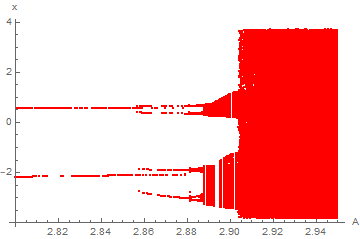
\includegraphics[width=0.5\linewidth]{plot/bif}
	\caption{bifurcation}
	\label{fig:bif 7}
\end{figure}

An important property of bifurcation plot is that the limiting ratio of each bifurcation interval to the next converge. so we can define the Feigenaum constant.
\begin{equation}
Q = \lim_{n \to \infty}\ \frac{a_{n-1}-a_{n-2}}{a_{n}-a_{n-1}}
\end{equation}
where $a_j$means the point where the period of motion doubles.[3] so we can define the Feigenbaum constant. In our system, the Feigenbaum's constant can only be calculated by approximation. As we can make the calculation $ (a_2-a_1)/(a_3-a_2)\approx0.025/0.006\approx4.17$ 
And it is quite similar to the theoretical value in limiting case, which is 4.669201.


\section{\textbf{CONCLUSIONS}}
From the above result, we can see that the amplitude of driven force(A) mainly affect the nonlinear behavior. In phase and time-series plots, we can see that transition between linearity and chaos do occur. We can know from experiment that the transition regime and critical point are between 4.5V and 8.7V, while from simulation they are between 1 and 3. When A is in transition regime, the sensitivity to the initial condition is shown by basin of attraction clearly. And a tiny change in initial value phase space often lead to completely different results afterward.Further surveys are added to precisely get the critical point, and that's what we do in Poincaré section and Periodic doubling. Finally we get the critical point near to 2.903 in the simulation. 

\textbf{References}

\bibliography{lab_report_1}
1.ANU.(2018).PHYS2017/2201 SECOND YEAR LABORATORY MANUAL. Canberra

2.The duffing equation, http://physics.ucsc.edu/~peter/115/duffing.pdf,n.d.

3.A PRECISE CALCULATION OF THE FEIGENBAUM CONSTANTS,KEITH BRIGGS. Mathematics of Computation. American Mathematical Society. 57 (195): 435–439.

4.https://mathematica.stackexchange.com/questions/136204/basins-of-attraction-for-the-duffing-equation-with-no-forcing-term/136483,n.d.


\appendix{\textbf{Appendix:Mathematica code}}
\begin{figure}[h]
	\centering
	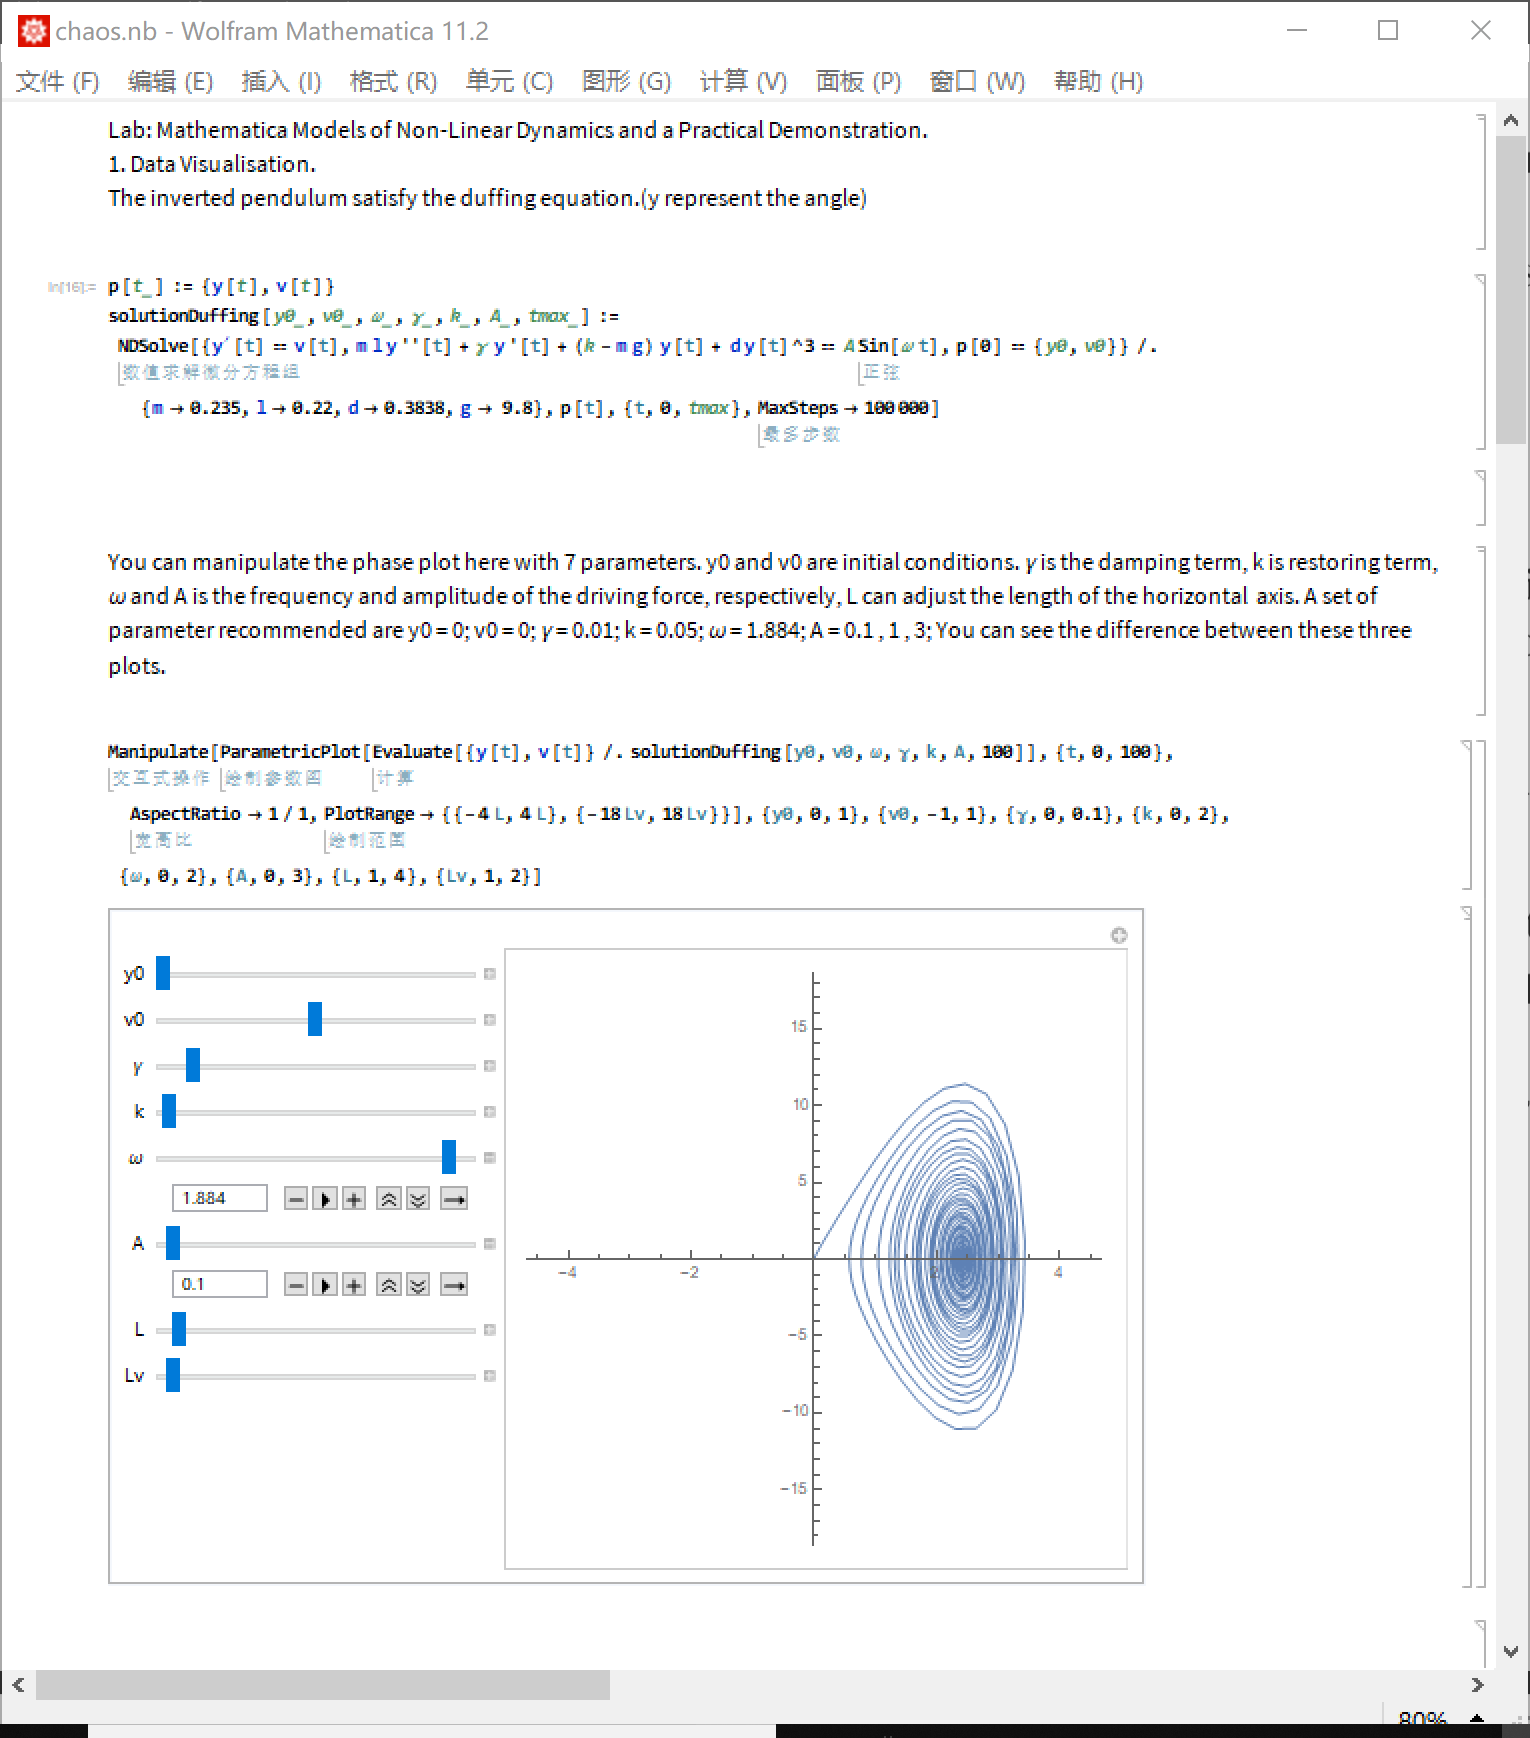
\includegraphics[width=0.6\linewidth]{plot/code1}
	\caption{Mathematica code 1}
	\label{fig:code1}
\end{figure}
\begin{figure}[h]
	\centering
	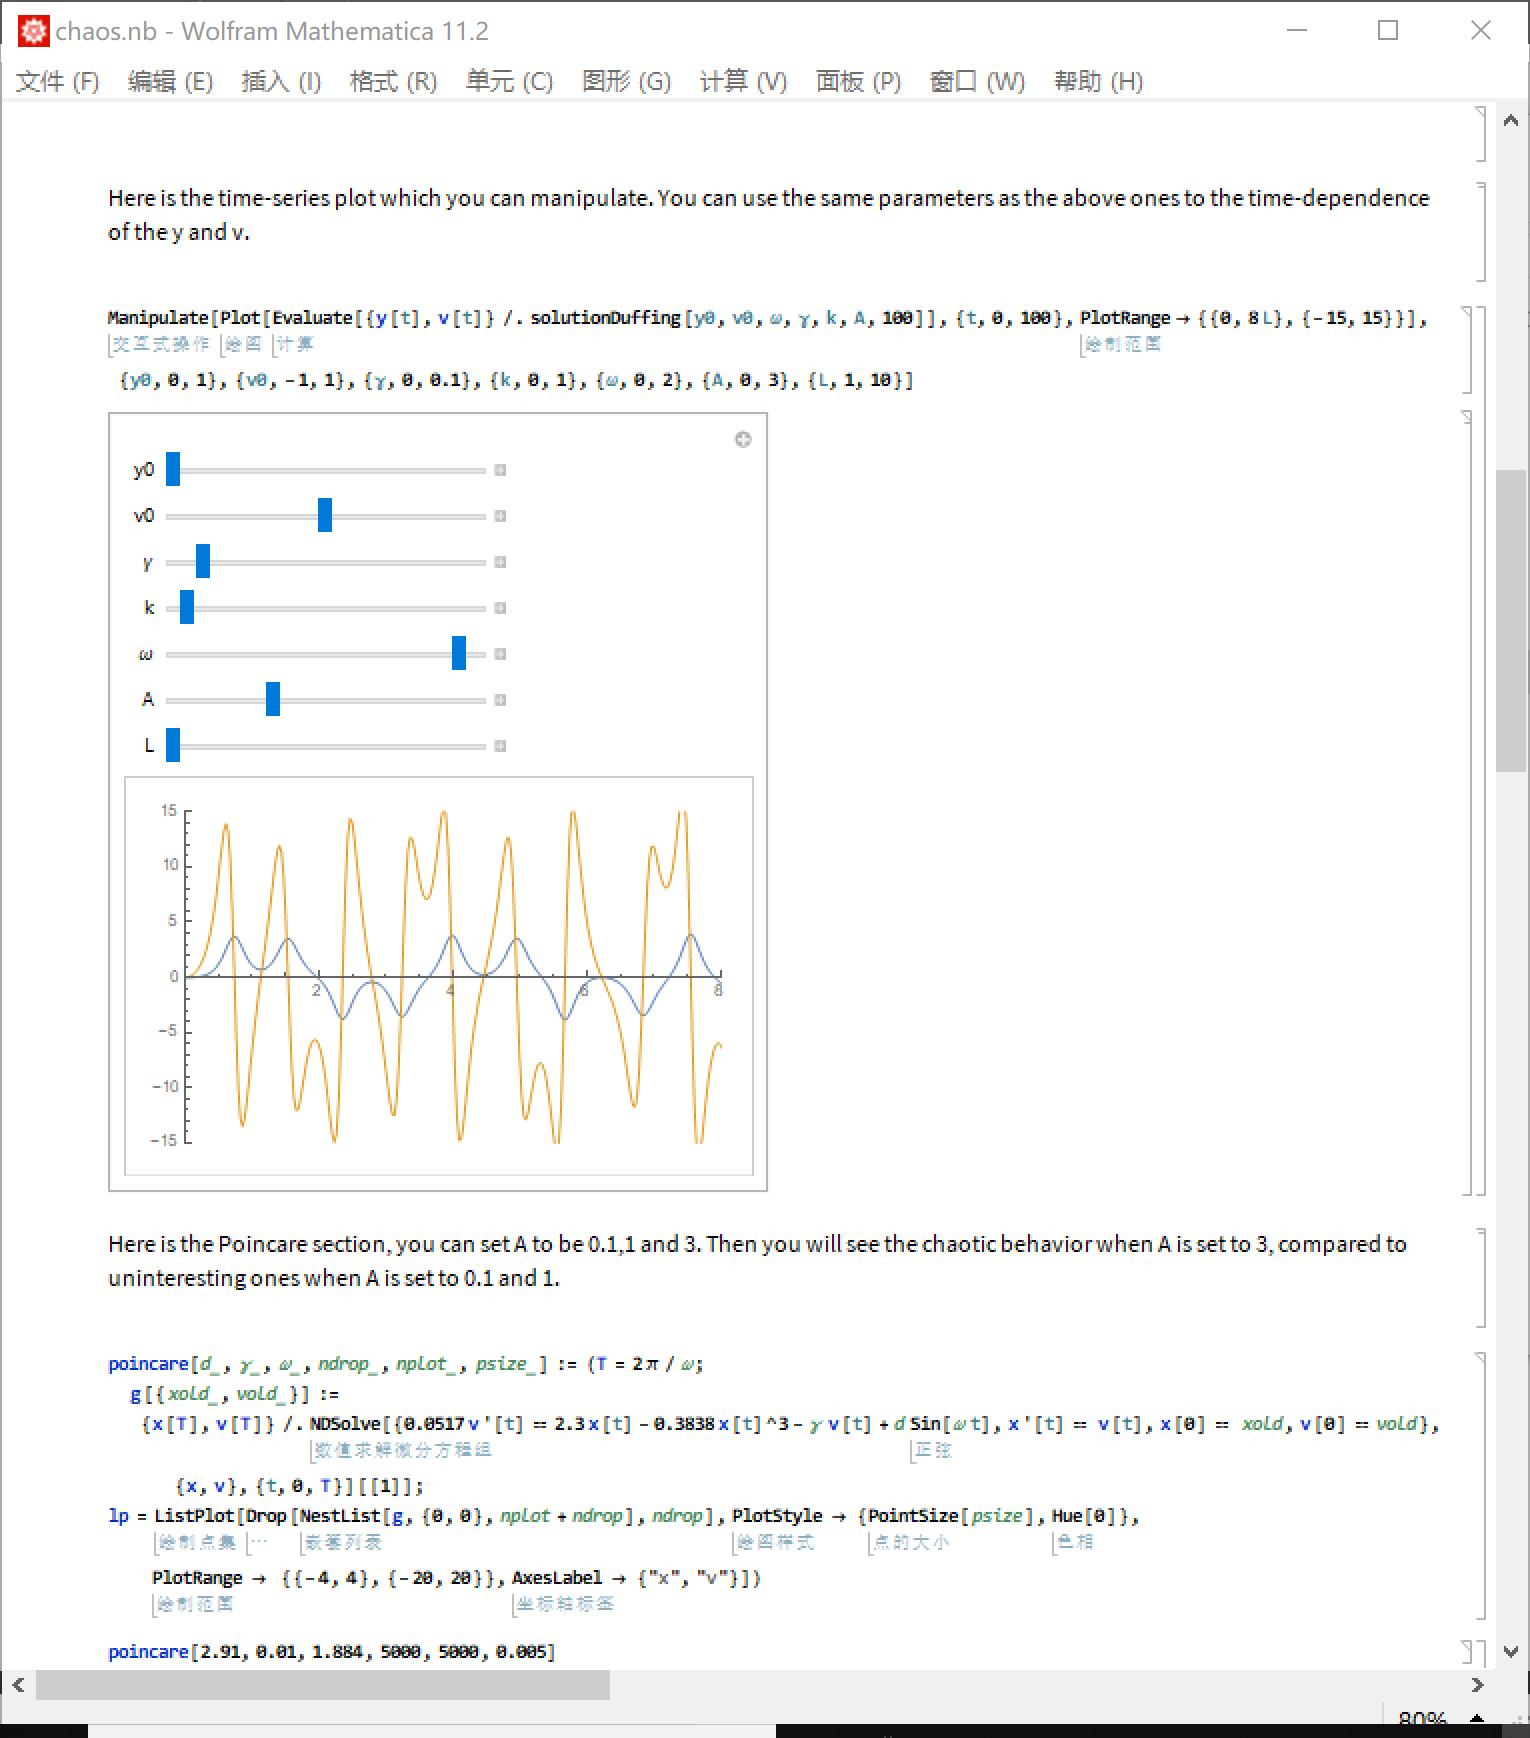
\includegraphics[width=0.6\linewidth]{plot/code2}
	\caption{Mathematica code 2}
	\label{fig:code2}
\end{figure}
\begin{figure}
	\centering
	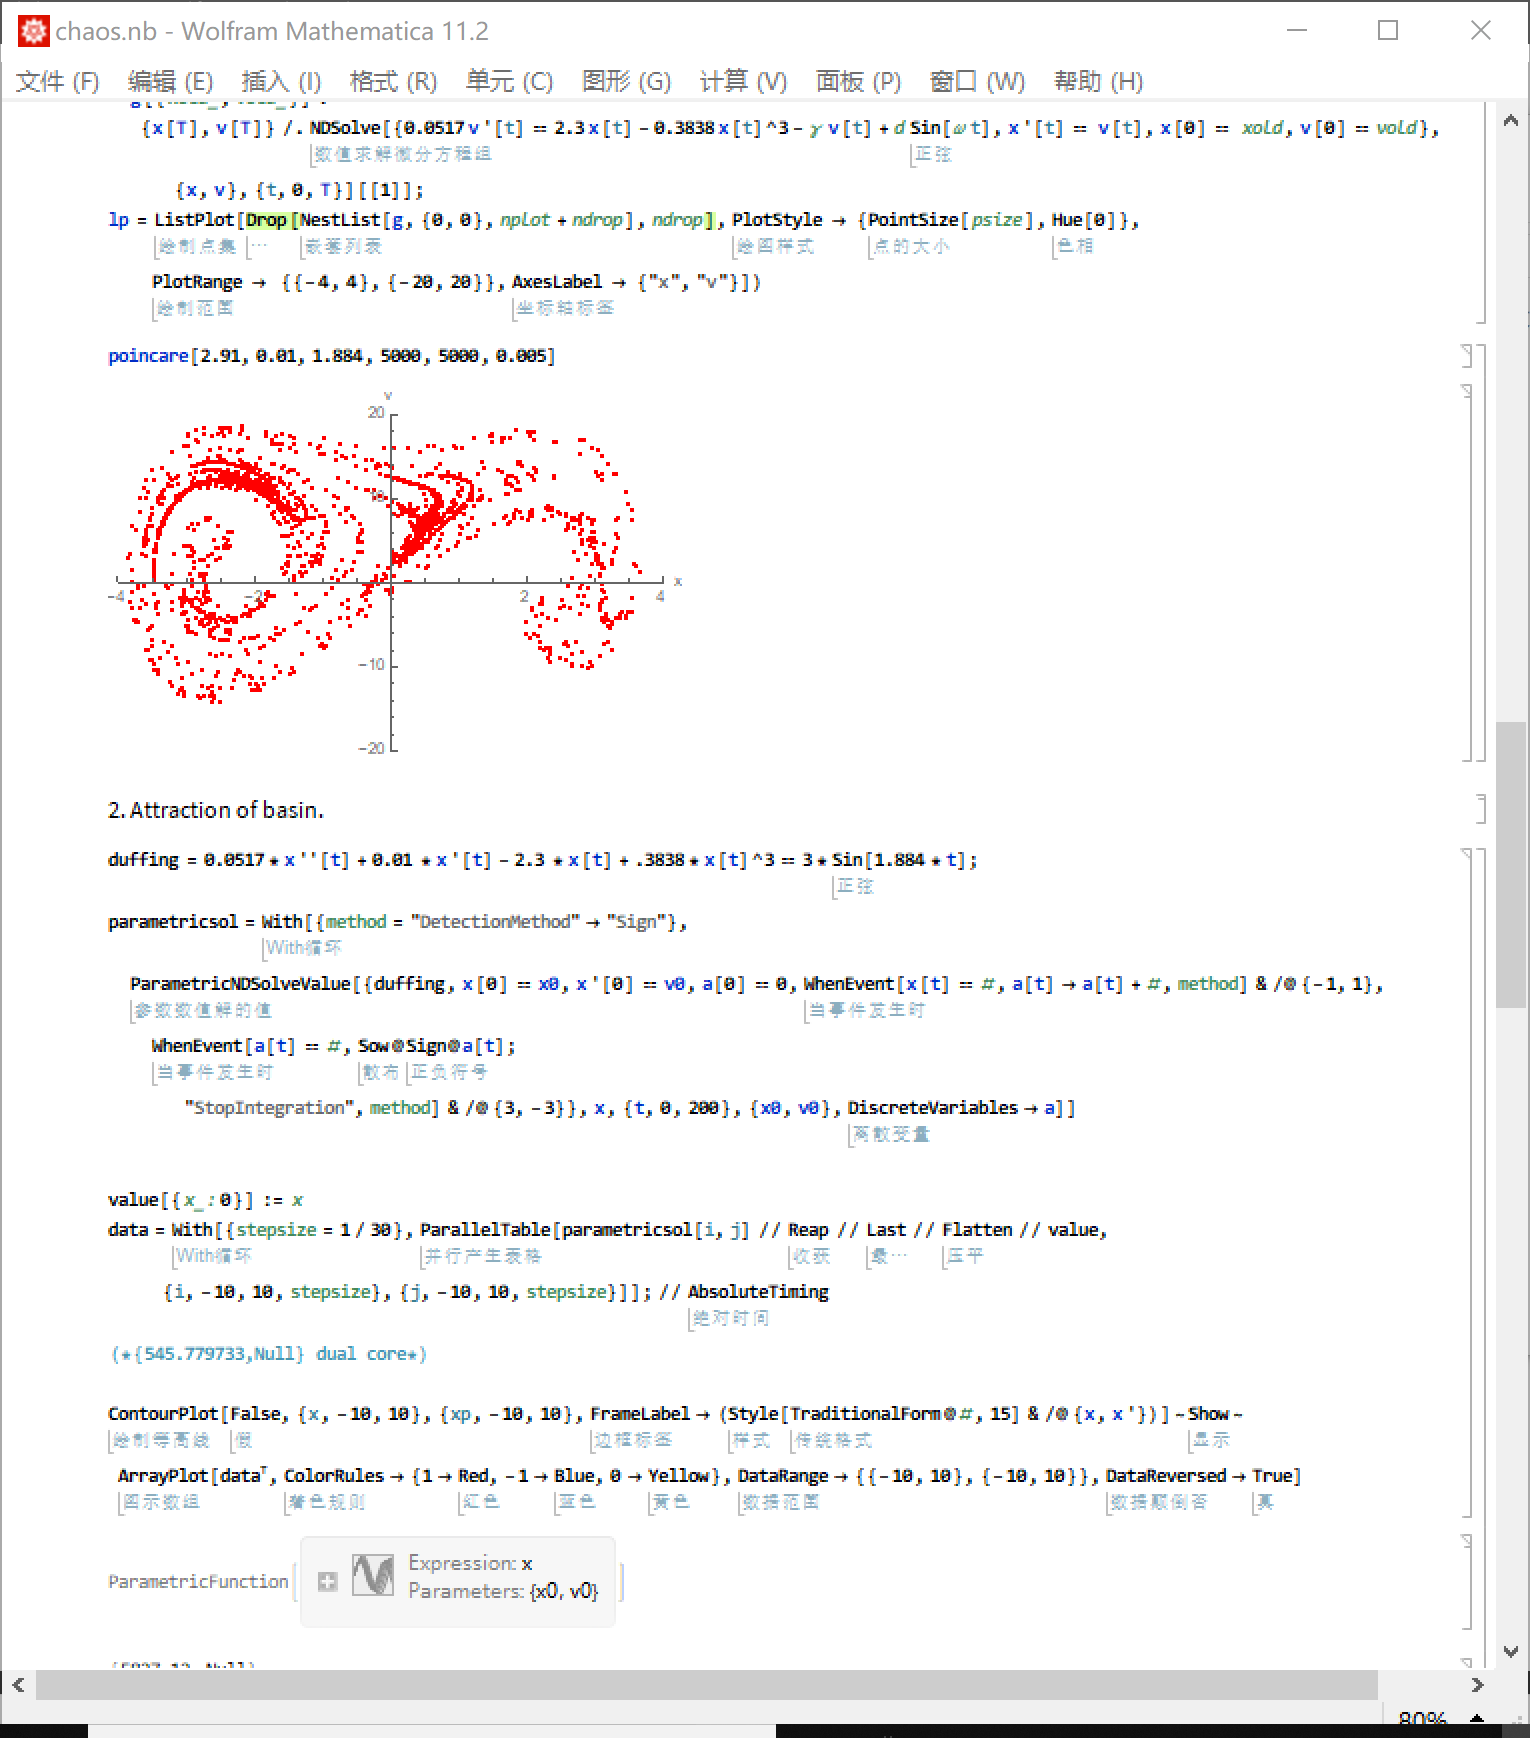
\includegraphics[width=0.6\linewidth]{plot/code3}
	\caption{Mathematica code 3}
	\label{fig:code3}
\end{figure}
\begin{figure}
	\centering
	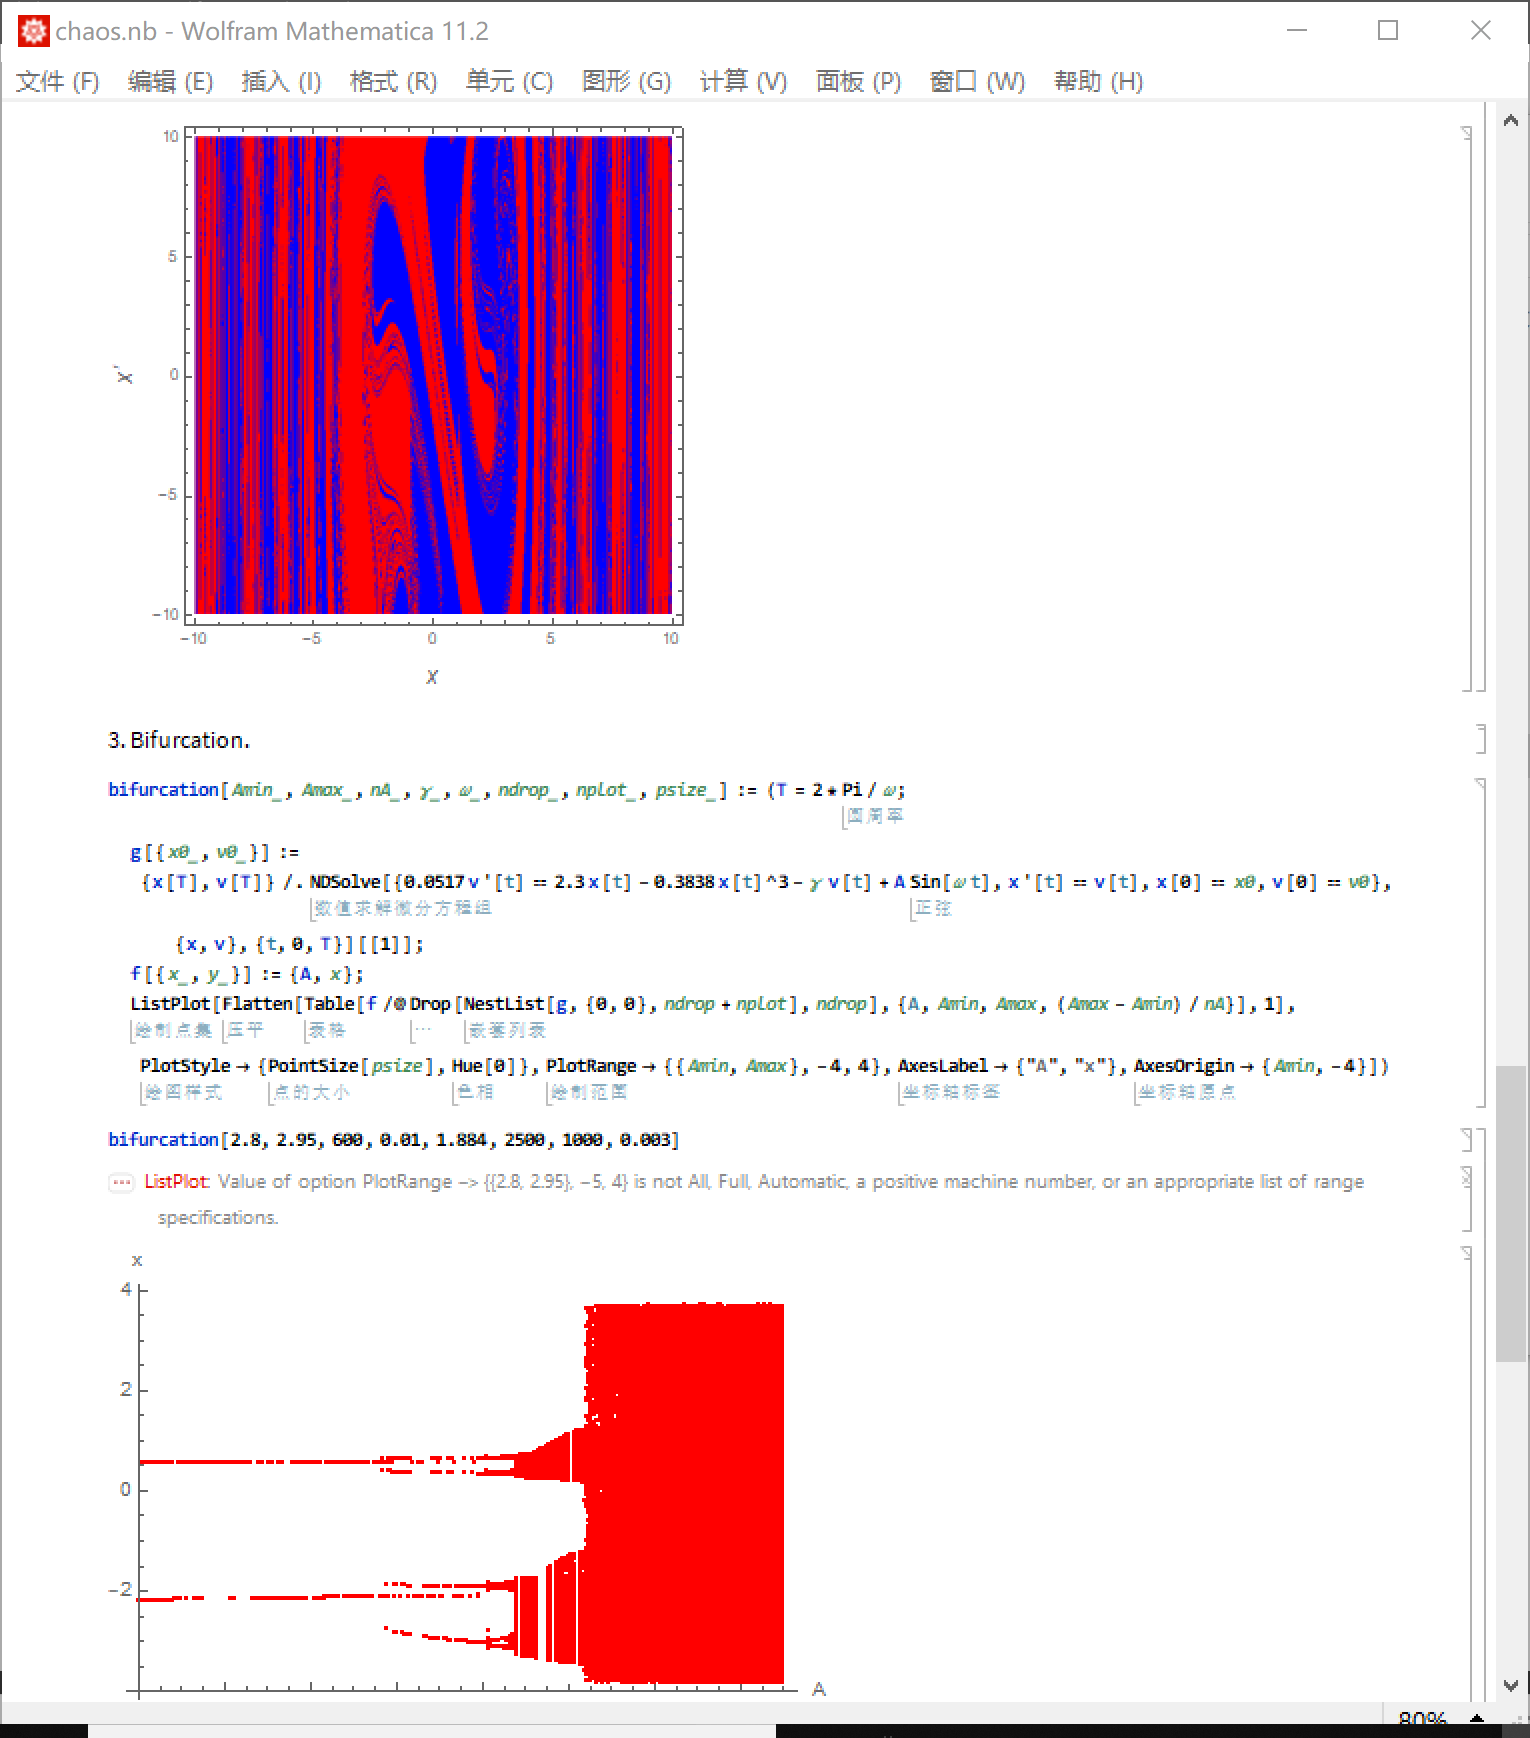
\includegraphics[width=0.6\linewidth]{plot/code4}
	\caption{Mathematica code 4}
	\label{fig:code4}
\end{figure}


\end{document}